\documentclass[12pt]{article}

\usepackage{sbc-template}
\usepackage[utf8]{inputenc}
\usepackage[T1]{fontenc}
\usepackage[brazilian]{babel}
\usepackage{graphicx,url}
\usepackage{booktabs}
\usepackage{array}
\usepackage{amsmath}

\sloppy

\title{Análise Experimental de Indexação, Planos de Execução e\\ Otimização de Consultas no Microsoft SQL Server 2022}

\author{Hermeson A., João Marcos R., Lizzandro W.,\\ Marcos W., Raildom R.\thanks{Projeto final da disciplina de Banco de Dados II (2026.2), ministrada pelo Prof. Dennis Sávio.}}

\address{Curso de Bacharelado em Sistemas de Informação\\
  Universidade Federal do Piauí (UFPI) -- CSHNB -- Picos -- PI -- Brasil}

\begin{document}

\maketitle

\begin{abstract}
Relational query performance depends on B+ Tree access paths and cost-based execution plans. This paper evaluates indexing, query rewriting, and execution plans on SQL Server 2022 over a 6.25-million-row e-commerce schema. Twin databases---a Baseline without secondary indexes and an Optimized counterpart with nine indexes---are compared across ten read queries and one batch write workload under Warm ($N=30$) and Cold ($N=10$) cache. Selective indexes, covering indexes, sargability, and \texttt{NOT EXISTS} reduced logical reads by up to 99.96\% ($>424\times$ speedup). Conversely, Q7 showed Batch Mode Hash Aggregation beating Row Mode Stream Aggregation in latency, while batch inserts (W1) added 85.33\% I/O overhead.
\end{abstract}

\begin{resumo}
O desempenho de consultas em bancos relacionais depende de caminhos em árvores B+ e planos físicos baseados em custos. Este artigo avalia indexação, reescrita lógica e planos no SQL Server 2022 em uma base de comércio eletrônico com 6,25 milhões de registros. Duas bases gêmeas --- Baseline (sem índices secundários) e Otimizada (nove índices) --- são comparadas em dez leituras e uma escrita em lote sob \textit{Warm} ($N=30$) e \textit{Cold} ($N=10$) \textit{cache}. Índices de cobertura, sargabilidade e \texttt{NOT EXISTS} reduziram leituras em até 99,96\% ($>424\times$). Porém, Q7 mostrou \textit{Hash Match} em \textit{Batch Mode} superando \textit{Stream Aggregate}, e W1 elevou o E/S em 85,33\%.
\end{resumo}

\section{Introdução}

À medida que sistemas transacionais e analíticos acumulam milhões de registros, o custo de entrada e saída (E/S) em disco e a varredura sequencial de páginas de memória tornam-se os principais gargalos de desempenho em Sistemas Gerenciadores de Bancos de Dados (SGBDs) relacionais. Mesmo em ambientes dotados de memória principal abundante e unidades SSD, operações de leitura integral de tabelas (\textit{Table/Clustered Scan}) degradam a latência de resposta, consomem largura de banda do \textit{buffer pool} e limitam a escalabilidade concorrente das aplicações \cite{silberschatz:20,ramakrishnan:03}.

A mitigação desses gargalos envolve duas frentes complementares: o projeto físico por meio de árvores B+ e a otimização de consultas baseada em custos (\textit{Cost-Based Optimization}) \cite{selinger:79,chaudhuri:98}. Contudo, índices secundários não são gratuitos: exigem espaço em disco, estatísticas atualizadas e manutenção síncrona em inserções, atualizações e remoções (\textit{write amplification}), penalizando cargas OLTP intensivas em escrita \cite{comer:79,elmasri:16}. Adicionalmente, predicados não \textit{sargable} (\textit{Search ARGument ABLE}) inviabilizam índices existentes, forçando varreduras integrais.

Este trabalho investiga experimentalmente o impacto real de estratégias de indexação, reescrita SQL e operadores físicos no Microsoft SQL Server 2022. Sobre uma base determinística de comércio eletrônico B2C com 6.250.000 registros, estruturamos duas bases gêmeas --- \texttt{Ecommerce\_Baseline} (apenas PKs clusterizadas) e \texttt{Ecommerce\_Otimizado} (nove índices secundários). As contribuições centrais são: (i) uma suíte reprodutível de onze cargas ($Q_1$--$Q_{10}$ e $W_1$) sob \textit{Warm Cache} ($N=30$) e \textit{Cold Cache} ($N=10$); (ii) o isolamento em três estágios do custo de \textit{Key Lookup} e sua eliminação via \texttt{INCLUDE}; e (iii) a análise empírica de \textit{write amplification} ($W_1$) e da inversão de latência entre \textit{Batch Mode on Rowstore} e \textit{Row Mode} em $Q_7$. A Seção~2 revisa a teoria; a Seção~3 detalha a metodologia; a Seção~4 discute os resultados; e a Seção~5 conclui o artigo.

\section{Referencial Teórico}

\subsection{Árvores B+ e Estratégias Avançadas de Indexação}

A estrutura padrão adotada por SGBDs relacionais comerciais para indexação ordenada em disco e memória paginada é a árvore B+ \cite{comer:79,elmasri:16}. Diferentemente de árvores binárias ou árvores B clássicas, a árvore B+ armazena todos os ponteiros ou registros de dados exclusivamente nos nós folha, mantendo nos nós internos apenas chaves de roteamento e ponteiros para subárvores. Essa separação maximiza o fator de ramificação (\textit{fan-out}) $m$ em páginas de tamanho fixo (8~KB no SQL Server), garantindo que a altura da árvore cresça apenas logaritmicamente ($O(\log_m N)$) e que buscas pontuais exijam tipicamente entre 2 e 4 acessos a páginas mesmo em tabelas com milhões de tuplas.

Nos índices \textbf{clusterizados} (\textit{Clustered Index}), os nós folha da árvore B+ contêm as próprias linhas de dados ordenadas fisicamente pela chave primária. Como consequência, uma tabela comporta apenas um índice clusterizado. Já nos índices \textbf{não-clusterizados} (\textit{Nonclustered Index}), cada entrada folha armazena a chave de busca acompanhada de um localizador para a linha completa --- no caso de tabelas com índice clusterizado, a própria chave clusterizada (\textit{Clustered Key}) \cite{microsoft:22}.

Quando uma consulta solicita colunas ausentes no índice não-clusterizado selecionado, o motor precisa executar um operador \textbf{Key Lookup} (junção em laço aninhado contra a árvore clusterizada) para cada registro qualificado. Se a seletividade do filtro for moderada, centenas ou milhares de buscas aleatórias por \textit{Key Lookup} acumulam leituras lógicas rapidamente, levando o otimizador a preferir um \textit{Clustered Index Scan} integral. Para eliminar esse custo, emprega-se o \textbf{Índice de Cobertura} (\textit{Covering Index}), que anexa colunas não-chave apenas ao nível folha mediante a cláusula \texttt{INCLUDE}. Essa técnica satisfaz integralmente projeções e filtros diretamente no índice secundário sem acessar a tabela base \cite{silberschatz:20}.

Outras duas especializações relevantes são os \textbf{índices compostos} e os \textbf{índices filtrados}. Em chaves compostas $(K_1, K_2)$, a ordem das colunas é determinante: os registros são ordenados primeiramente por $K_1$ e, dentro de cada valor distinto de $K_1$, por $K_2$. Logo, predicados combinando igualdade em $K_1$ e faixa (\textit{range}) em $K_2$ realizam um único \textit{Index Seek} contíguo, enquanto a ordem inversa degradaria o acesso para varreduras parciais \cite{ramakrishnan:03}. Já os índices filtrados (\texttt{CREATE INDEX ... WHERE}) indexam apenas o subconjunto de tuplas relevante a um predicado seletivo, reduzindo tamanho em disco, profundidade da árvore e custo de manutenção em escrita \cite{microsoft:22}. Em contrapartida, toda instrução \texttt{INSERT}, \texttt{UPDATE} ou \texttt{DELETE} exige a atualização síncrona de cada árvore B+ afetada, gerando acréscimo proporcional de leituras lógicas, contenção de \textit{log} e eventuais divisões de páginas (\textit{page splits}).

\subsection{Otimização Baseada em Custos e Operadores Físicos}

Desde a arquitetura pioneira do System~R \cite{selinger:79} até otimizadores modernos baseados nas arquiteturas Volcano/Cascades \cite{graefe:93,chaudhuri:98}, a compilação de uma consulta SQL percorre etapas de análise léxica/sintática, normalização lógica e enumeração de planos físicos orientada por um modelo de custos de E/S e CPU. Para que o otimizador substitua algoritmos de custo $O(N)$ (como \textit{Clustered Scan}) por caminhos sublineares $O(\log N + k)$ (\textit{Index Seek}), o predicado deve preservar a propriedade de \textbf{sargabilidade}: a coluna indexada deve figurar isolada em um dos lados do operador relacional. Expressões como \texttt{YEAR(DataPedido) = 2025} ou \texttt{LIKE N'\%Notebook\%'} inviabilizam a busca binária na árvore B+ porque exigem a avaliação da função sobre toda a coluna, enquanto intervalos semiabertos (\texttt{>= '2025-01-01' AND < '2026-01-01'}) e buscas por prefixo (\texttt{LIKE N'Notebook\%'}) restauram o \textit{Index Seek}. Analogamente, subconsultas correlacionadas com agregação podem frequentemente ser reescritas com \texttt{NOT EXISTS}, habilitando planos \textit{Left Anti Semi Join} mais econômicos.

A enumeração de junções combina três algoritmos físicos clássicos \cite{graefe:93,ramakrishnan:03}: (i) \textbf{Nested Loops Join}, eficiente quando a entrada externa é pequena e a interna dispõe de índice seletivo; (ii) \textbf{Merge Join}, de complexidade linear quando ambas as entradas já chegam ordenadas pelos respectivos índices; e (iii) \textbf{Hash Match Join}, adequado a grandes volumes não ordenados mediante construção de tabela \textit{hash} em memória (sujeita a \textit{memory grant} e eventual \textit{spill} em \texttt{tempdb}).

Um aspecto crucial dos motores modernos --- presente no SQL Server 2019 e 2022 --- é o processamento em lote sobre armazenamento orientado a linhas (\textbf{Batch Mode on Rowstore}). Em consultas analíticas e agregações sobre grandes tabelas, operadores como \textit{Hash Match} e varreduras podem processar vetores de até 900 tuplas por bloco com menor sobrecarga de chamadas virtuais por linha, reduzindo drasticamente o tempo de CPU em comparação ao modelo tradicional iterador tupla-a-tupla (\textit{Row Mode}) \cite{graefe:93,microsoft:22}. Assim, um plano com menor número de leituras lógicas em \textit{Row Mode} pode, paradoxalmente, apresentar maior latência de CPU do que uma varredura vetorizada em \textit{Batch Mode}.

\section{Metodologia Experimental}

\subsection{Ambiente Computacional, Esquema e Bases Gêmeas}

Todos os experimentos foram conduzidos em ambiente conteinerizado reprodutível sobre \textit{host} Windows~11 Home Single Language equipado com processador Intel Core i5-1235U (12ª geração, 10 núcleos / 12 threads), 15,71~GB de RAM e armazenamento SSD. O SGBD avaliado foi o \textbf{Microsoft SQL Server 2022 RTM-CU28} (versão 16.0.4325.4, \textit{Developer Edition} 64-bit) executando em container Docker (Ubuntu 22.04.5 LTS) com limite de 4~GB de memória. A orquestração em Python 3 (gerenciada via \texttt{uv}) conectou-se ao motor por meio da biblioteca \texttt{pymssql}.

Projetou-se um esquema relacional normalizado de comércio eletrônico B2C composto por quatro tabelas povoadas deterministicamente (\textit{seed}~42, com distribuições sintéticas realistas incluindo ~20\% de itens com desconto elevado $\ge 10{,}00$): \texttt{Clientes} (200.000 linhas), \texttt{Produtos} (50.000 linhas), \texttt{Pedidos} (1.500.000 linhas) e \texttt{ItensPedido} (4.500.000 linhas), totalizando \textbf{6.250.000 registros} (400~MB alocados na base, com 259.064~KB em dados e 272.216~KB reservados) sob modelo de recuperação \texttt{SIMPLE}.

Após a carga massiva e atualização completa de estatísticas (\texttt{sp\_updatestats}) em \texttt{Ecommerce\_Baseline} --- que preserva estritamente as 4 chaves primárias clusterizadas e nenhuma indexação secundária --- realizou-se \texttt{BACKUP} e \texttt{RESTORE} com isolamento de arquivos para gerar a base gêmea \texttt{Ecommerce\_Otimizado}. Verificou-se integridade referencial confiável (\texttt{is\_not\_trusted = 0}) e paridade absoluta nas 12 estatísticas iniciais entre ambas as bases antes da criação dos nove índices secundários resumidos na Tabela~\ref{tab:indices}.

\begin{table}[ht]
\centering
\caption{Índices secundários não-clusterizados implantados exclusivamente em \texttt{Ecommerce\_Otimizado} (amostragem estatística de 100\% em todos os índices).}
\label{tab:indices}
\scriptsize
\setlength{\tabcolsep}{3pt}
\begin{tabular}{@{}lp{3.5cm}p{4.2cm}l@{}}
\toprule
\textbf{Índice} & \textbf{Tabela (Chave)} & \textbf{Colunas \texttt{INCLUDE} / Filtro} & \textbf{Alvo} \\
\midrule
\texttt{IX\_Clientes\_Email} & \texttt{Clientes (Email)} & -- & $Q_1$ \\
\texttt{IX\_Produtos\_Nome} & \texttt{Produtos (Nome)} & \texttt{INCLUDE (Categoria, Preco)} & $Q_8$ \\
\texttt{IX\_Pedidos\_DataPedido} & \texttt{Pedidos (DataPedido)} & \texttt{INCLUDE (ClienteID, Status, ValorTotal)} & $Q_2, Q_6, Q_9$ \\
\texttt{IX\_Pedidos\_Status\_Data} & \texttt{Pedidos (Status, DataPedido)} & -- & $Q_3$ \\
\texttt{IX\_Pedidos\_ClienteID\_Cov} & \texttt{Pedidos (ClienteID)} & \texttt{INCLUDE (DataPedido, ValorTotal)} & $Q_4, Q_5, Q_{10}$ \\
\texttt{IX\_Pedidos\_Status\_Cov} & \texttt{Pedidos (Status)} & \texttt{INCLUDE (ValorTotal)} & $Q_7$ \\
\texttt{IX\_ItensPedido\_PedidoID} & \texttt{ItensPedido (PedidoID)} & \texttt{INCLUDE (ProdutoID, Quantidade, PrecoUnitario)} & $Q_5, W_1$ \\
\texttt{IX\_ItensPedido\_ProdutoID} & \texttt{ItensPedido (ProdutoID)} & -- & $W_1$ \\
\texttt{IX\_ItensPedido\_Desconto\_Alto} & \texttt{ItensPedido (ProdutoID, Desconto)} & \texttt{WHERE Desconto >= 10.00} (901.180 linhas) & Seletivo / $W_1$ \\
\bottomrule
\end{tabular}
\end{table}

\subsection{Carga de Trabalho e Protocolo Estatístico}

A carga experimental compreende dez consultas de leitura ($Q_1$--$Q_{10}$) e uma carga de inserção em lote ($W_1$), sumarizadas na Tabela~\ref{tab:workload}. Para isolar o efeito das estruturas de acesso e evitar flutuações de escalonamento paralelo entre threads em uma instância conteinerizada, todas as consultas empregaram \texttt{OPTION (MAXDOP 1)} e literais tipados compatíveis (prevenindo conversões implícitas). Na consulta $Q_4$, capturou-se ainda um estágio intermediário com índice simples \texttt{IX\_Pedidos\_ClienteID} (sem \texttt{INCLUDE}) antes de sua substituição por \texttt{IX\_Pedidos\_ClienteID\_Cov}, quantificando o impacto isolado do \textit{Key Lookup}.

\begin{table}[ht]
\centering
\caption{Resumo da carga experimental ($Q_1$--$Q_{10}$ e $W_1$) e transformações aplicadas no cenário otimizado.}
\label{tab:workload}
\scriptsize
\setlength{\tabcolsep}{3pt}
\begin{tabular}{@{}lp{4.1cm}p{5.5cm}r@{}}
\toprule
\textbf{Cód.} & \textbf{Descrição Funcional} & \textbf{Estratégia Aplicada (Baseline $\rightarrow$ Otimizado)} & \textbf{Linhas} \\
\midrule
$Q_1$ & Busca pontual por e-mail & Índice simples (\textit{Scan} $\rightarrow$ \textit{Index Seek + Lookup}) & 1 \\
$Q_2$ & Faixa restrita de datas & Índice com cobertura (\textit{Scan} $\rightarrow$ \textit{Index Seek}) & 6.028 \\
$Q_3$ & \texttt{Status} + faixa \texttt{DataPedido} & Índice composto ordenado (\texttt{Status, DataPedido}) & 3.198 \\
$Q_4$ & Pedidos de um cliente & Eliminação de \textit{Lookup} via \textit{Covering Index} & 422 \\
$Q_5$ & Junção de 3 tabelas & \textit{Hash Match} duplo $\rightarrow$ \textit{Merge} + \textit{Nested Loops} & 4.965 \\
$Q_6$ & \texttt{TOP 50} pedidos recentes & Eliminação de \textit{Sort} via leitura reversa & 50 \\
$Q_7$ & Faturamento por \texttt{Status} & \textit{Hash Match [Batch]} $\rightarrow$ \textit{Stream Agg. [Row]} & 6 \\
$Q_8$ & Busca textual em catálogo & \texttt{LIKE N'\%Notebook\%'} $\rightarrow$ \texttt{LIKE N'Notebook\%'} & 2.002 \\
$Q_9$ & Total anual de pedidos (2025) & \texttt{YEAR(Data)=2025} $\rightarrow$ intervalo semiaberto & 1 \\
$Q_{10}$ & Clientes sem pedidos & Subconsulta correlacionada $\rightarrow$ \texttt{NOT EXISTS} & 10.060 \\
$W_1$ & Inserção OLTP em lote & Controle de \textit{write amplification} em 3 índices sec. & 10.000 \\
\bottomrule
\end{tabular}
\end{table}

Cada cenário foi executado em dois regimes: (1) \textbf{\textit{Warm Cache}} ($N=30$ repetições pareadas por consulta, precedidas de 2 aquecimentos descartados e com alternância de ordem entre as bases por repetição para mitigar deriva térmica/OS); e (2) \textbf{\textit{Cold Cache}} ($N=10$ repetições, executando \texttt{CHECKPOINT; DBCC DROPCLEANBUFFERS; DBCC FREEPROCCACHE;} antes de cada medição para esvaziar o \textit{buffer pool} e o cache de planos). A carga de escrita $W_1$ foi encapsulada em \texttt{BEGIN TRANSACTION ... ROLLBACK TRANSACTION} garantindo contagem intacta de 4.500.000 linhas em \texttt{ItensPedido} e paridade absoluta de \texttt{row\_count} em todas as 880 medições. Extraíram-se métricas diretamente do motor via \texttt{SET STATISTICS IO, TIME ON} e planos reais via \texttt{SET STATISTICS XML ON}. Na inferência estatística, aplicou-se o teste de Shapiro-Wilk sobre as diferenças pareadas ($\alpha = 0{,}05$) para selecionar o teste $t$ de Student pareado (normalidade aceita) ou o teste de Wilcoxon pareado (não-paramétrico).

\section{Resultados e Discussão}

\subsection{Visão Geral em \textit{Warm Cache} ($N=30$) e Redução de E/S}

A Tabela~\ref{tab:resultados-warm} consolida os resultados medidos em \textit{Warm Cache} ($N=30$). Em nove das dez consultas de leitura ($Q_1$--$Q_6$, $Q_8$--$Q_{10}$), a combinação de índices seletivos e reescrita SQL reduziu significativamente ($p < 10^{-4}$) tanto o volume de páginas lidas em memória quanto a latência de execução. Como o temporizador interno do SQL Server possui resolução de 1~ms, tempos inferiores a 0,5~ms são reportados como 0~ms pelo SGBD; por transparência, tais casos ($Q_1$, $Q_4$ e $Q_6$) são anotados como $<1$~ms e têm aceleração conservadora expressa em relação ao limite de 1~ms (por exemplo, $>424\times$ em $Q_6$).

% Gerado automaticamente por scripts/analyze_results.py (Warm Cache N=30)
\begin{table}[ht]
\centering
\caption{Comparativo de desempenho em \textit{Warm Cache} ($N=30$): Leituras Lógicas, Tempo de Execução (mediana $\pm$ DP), Redução de E/S, \textit{Speedup} e significância estatística.}
\label{tab:resultados-warm}
\scriptsize
\setlength{\tabcolsep}{3.5pt}
\begin{tabular}{lrrrrrrr}
\toprule
\textbf{Cons.} & \textbf{Leit. Base} & \textbf{Leit. Otim.} & \textbf{Red. E/S} & \textbf{Tempo Base (ms)} & \textbf{Tempo Otim. (ms)} & \textbf{Speedup} & \textbf{$p$-valor} \\
\midrule
Q1 & 2.856 & 6 & 99,79\% & 15,0 $\pm$ 4,4 & $<1$ $\pm$ 0,0 & $>$15x ($<$1 ms) & $<10^{-4}$ \\
Q2 & 8.090 & 34 & 99,58\% & 104,5 $\pm$ 96,9 & 1,5 $\pm$ 1,8 & 69,7x & $<10^{-4}$ \\
Q3 & 8.090 & 17 & 99,79\% & 87,0 $\pm$ 17,5 & 1,0 $\pm$ 0,6 & 87,0x & $<10^{-4}$ \\
Q4 & 8.090 & 5 & 99,94\% & 111,0 $\pm$ 62,9 & $<1$ $\pm$ 0,3 & $>$111x ($<$1 ms) & $<10^{-4}$ \\
Q5 & 28.818 & 5.295 & 81,63\% & 450,0 $\pm$ 19,4 & 12,0 $\pm$ 2,4 & 37,5x & $<10^{-4}$ \\
Q6 & 8.090 & 3 & 99,96\% & 424,0 $\pm$ 25,0 & $<1$ $\pm$ 0,0 & $>$424x ($<$1 ms) & $<10^{-4}$ \\
\textbf{Q7} & 8.090 & 5.658 & 30,06\% & 217,0 $\pm$ 11,8 & 364,0 $\pm$ 36,0 & 0,60x & $<10^{-4}$ \\
Q8 & 637 & 28 & 95,60\% & 114,0 $\pm$ 3,6 & 1,0 $\pm$ 0,4 & 114,0x & $<10^{-4}$ \\
Q9 & 8.090 & 1.565 & 80,66\% & 226,0 $\pm$ 17,9 & 26,0 $\pm$ 1,8 & 8,69x & $<10^{-4}$ \\
Q10 & 10.946 & 8.252 & 24,61\% & 370,5 $\pm$ 34,2 & 219,5 $\pm$ 23,9 & 1,69x & $<10^{-4}$ \\
\midrule
\textbf{W1} & 97.154 & 180.057 & -85,33\% & 384,0 $\pm$ 113,9 & 404,0 $\pm$ 853,2 & 0,95x & 0,129 \\
\bottomrule
\end{tabular}
\end{table}


Conforme ilustrado na Figura~\ref{fig:leituras-logicas} (escala logarítmica), os maiores ganhos de E/S ocorreram nas consultas seletivas e ordenadas: $Q_6$ caiu de 8.090 para 3 páginas (-99,96\%), eliminando o \textit{Sort} via leitura reversa (\texttt{BACKWARD}) de \texttt{IX\_Pedidos\_DataPedido}; $Q_4$ reduziu 99,94\% (8.090 $\rightarrow$ 5 páginas); $Q_1$ e $Q_3$ em 99,79\%; e $Q_2$ em 99,58\% (8.090 $\rightarrow$ 34 páginas). Em $Q_8$, trocar \texttt{LIKE N'\%Notebook\%'} por \texttt{LIKE N'Notebook\%'} sobre \texttt{IX\_Produtos\_Nome} reduziu leituras em 95,60\% (637 $\rightarrow$ 28 páginas, $114{,}0\times$). Cabe ressaltar a alteração semântica dessa reescrita: o curinga inicial busca substrings arbitrárias, enquanto o prefixo limita-se ao início do texto, sendo válido no domínio apenas quando nomes de produtos seguem taxonomia padronizada iniciada pela categoria (caso desta base, com 2.002 linhas idênticas; textos livres exigiriam \textit{Full-Text}). Em $Q_9$, substituir \texttt{YEAR(DataPedido) = 2025} por intervalo semiaberto habilitou \textit{Index Seek} em \texttt{IX\_Pedidos\_DataPedido}, caindo de 8.090 para 1.565 páginas (-80,66\%, $8{,}69\times$).

\begin{figure}[htbp]
\centering
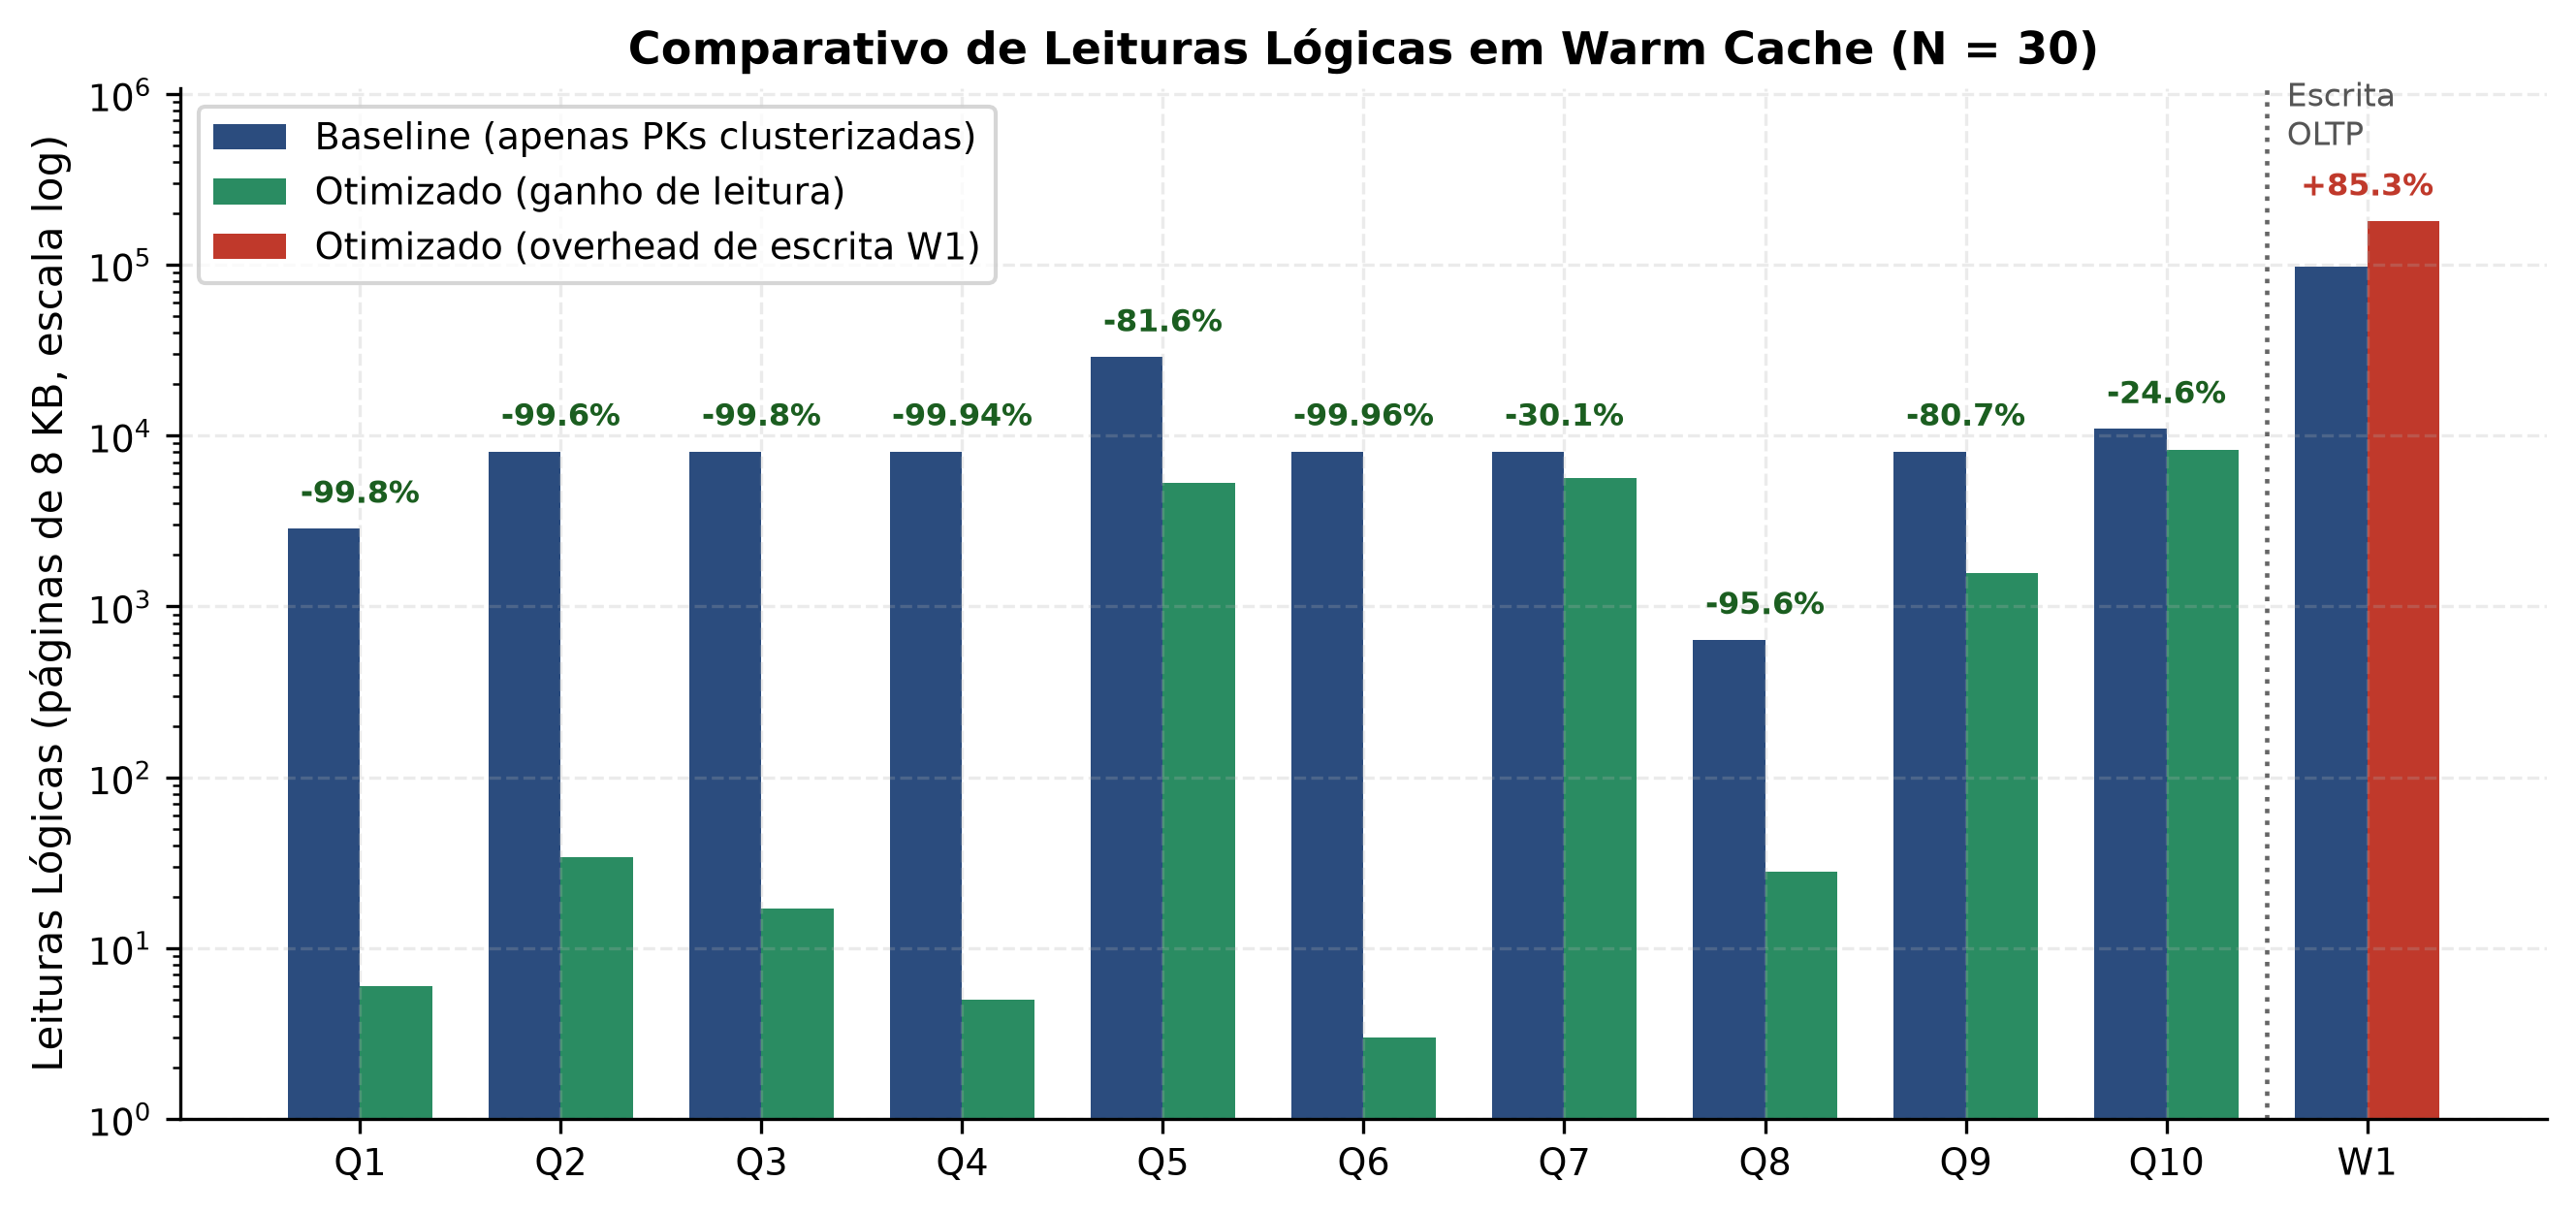
\includegraphics[width=0.73\textwidth]{figures/fig1_leituras_logicas.png}
\caption{Leituras lógicas medianas em \textit{Warm Cache} ($N=30$, escala logarítmica), evidenciando reduções de até 99,96\% nas leituras e o acréscimo de +85,3\% na escrita $W_1$.}
\label{fig:leituras-logicas}
\end{figure}

Nas consultas estruturalmente mais complexas ($Q_5$ e $Q_{10}$), os benefícios decorreram da alteração dos algoritmos físicos de junção. Em $Q_5$, o plano Baseline realizava duas varreduras completas em \texttt{Pedidos} (8.090 páginas) e \texttt{ItensPedido} (20.721 páginas) unidas por dois operadores \textit{Hash Match}, totalizando 28.818 páginas e 450,0~ms medianos. Com os índices de cobertura nas chaves estrangeiras, o otimizador substituiu o plano por um \textit{Merge Join} (entre \texttt{Clientes} e \texttt{Pedidos}) acoplado a um \textit{Nested Loops} com busca indexada em \texttt{IX\_ItensPedido\_PedidoID}, derrubando o tempo para 12,0~ms ($37{,}5\times$). Em $Q_{10}$, a reescrita da subconsulta correlacionada agregada para \texttt{NOT EXISTS} converteu o plano de um duplo \textit{Hash Match} + \textit{Filter} (10.946 páginas, 370,5~ms) para um \textit{Merge Join [Left Anti Semi Join]} com \textit{Stream Aggregate} sobre \texttt{IX\_Pedidos\_ClienteID\_Cov} (8.252 páginas, 219,5~ms, $1{,}69\times$). A Figura~\ref{fig:boxplots} detalha a baixa dispersão das latências otimizadas frente aos cenários Baseline.

\begin{figure}[htbp]
\centering
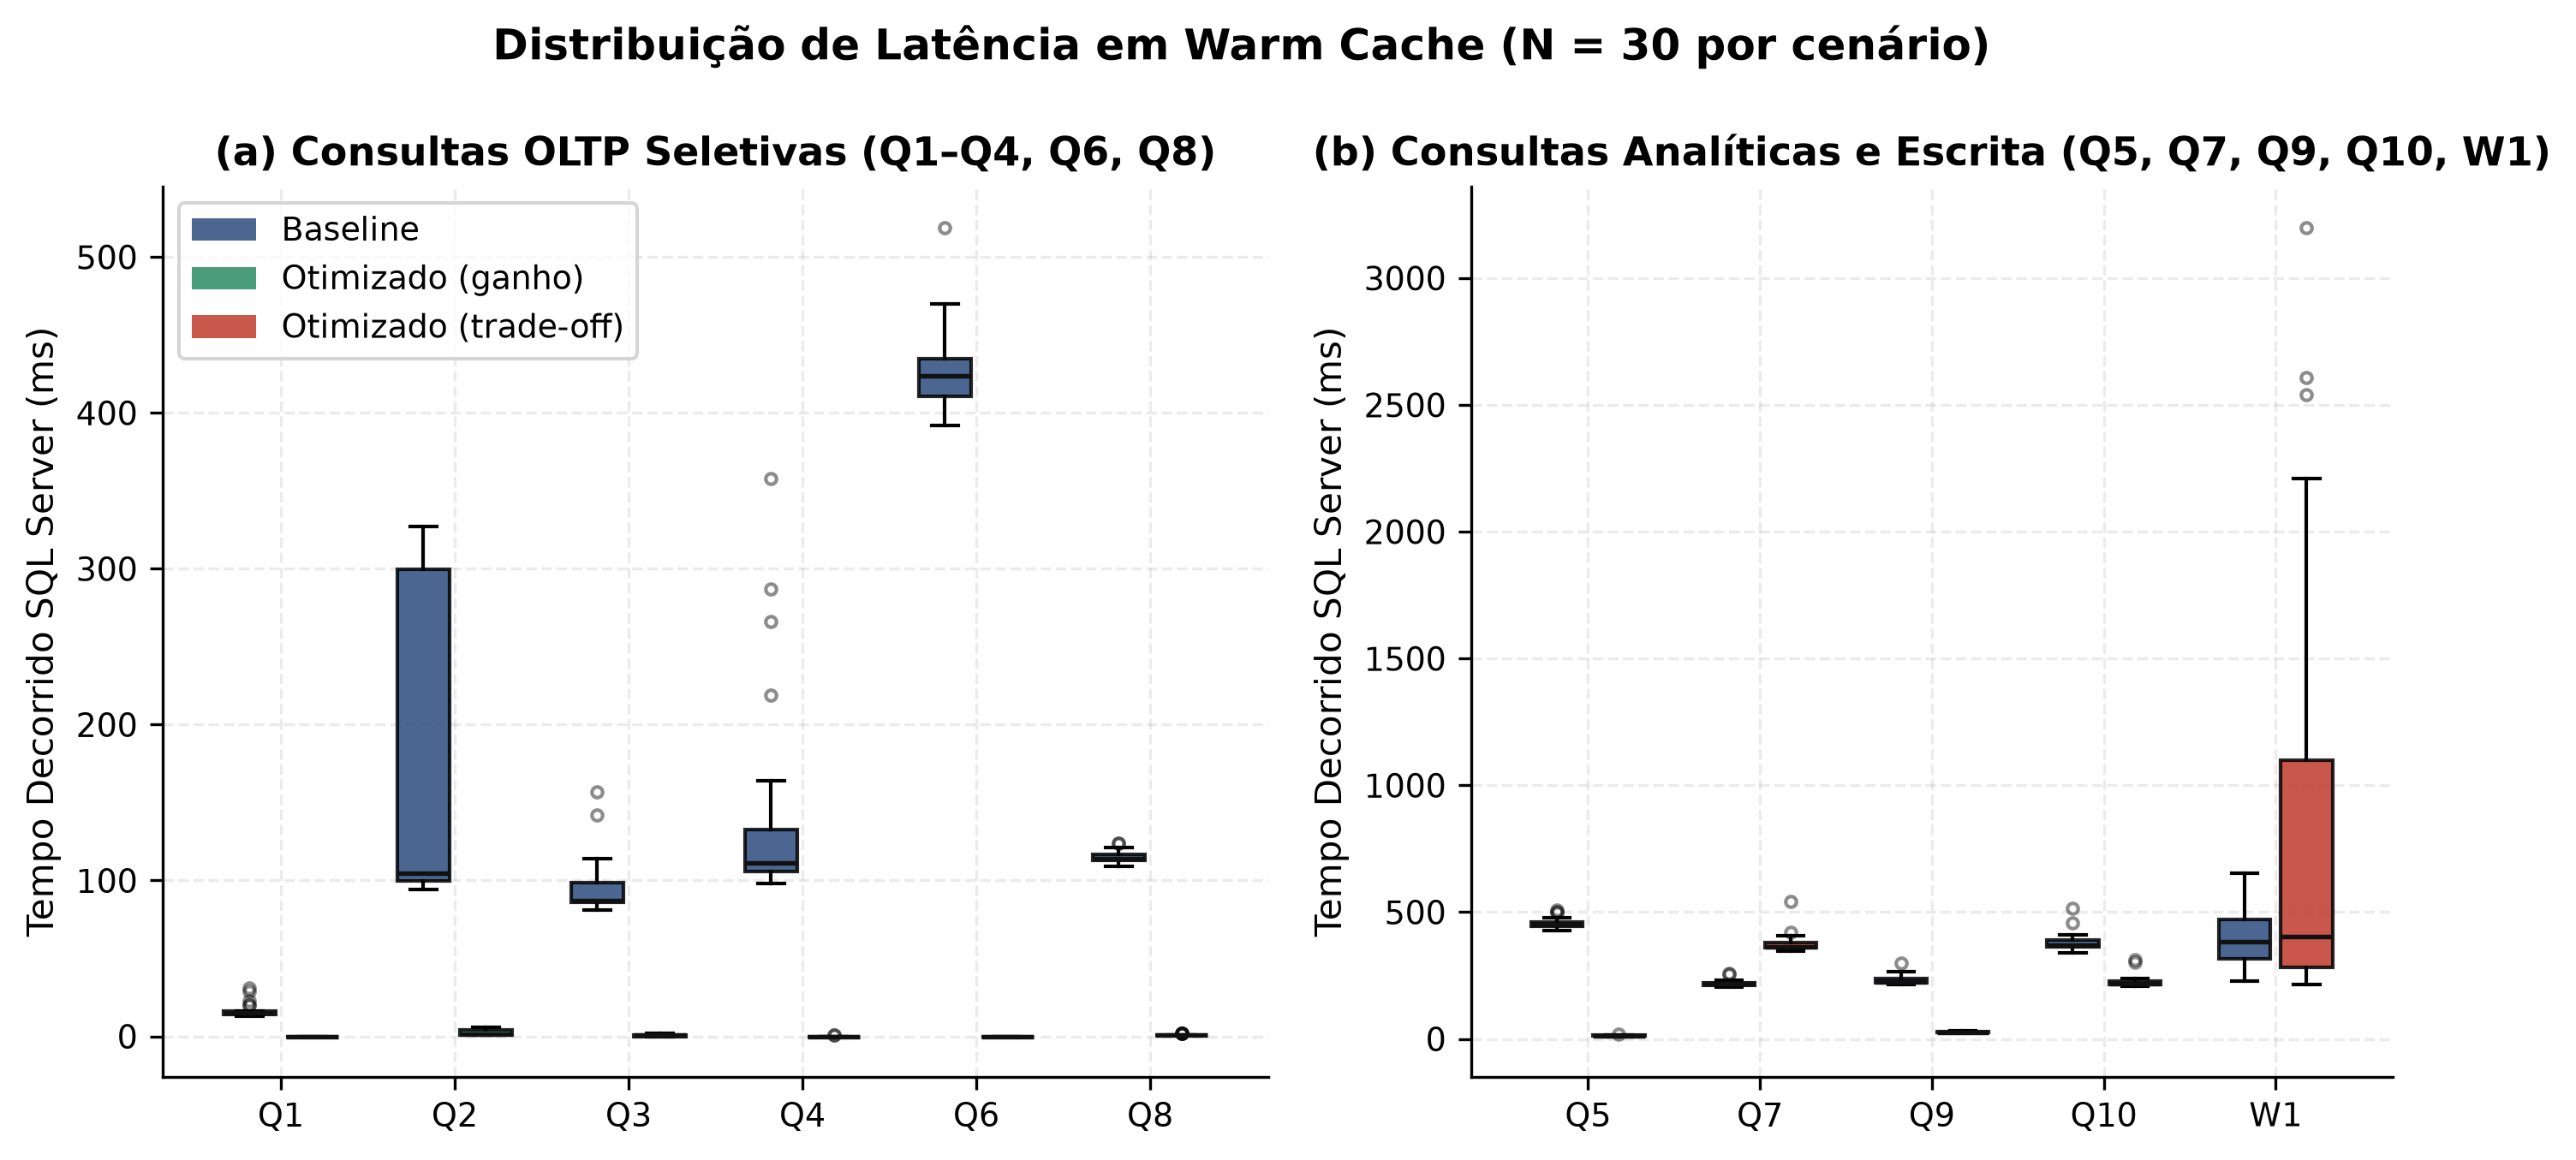
\includegraphics[width=0.79\textwidth]{figures/fig2_tempos_execucao_boxplot.png}
\caption{Distribuição dos tempos de execução em \textit{Warm Cache} ($N=30$) para consultas OLTP seletivas (a) e consultas analíticas/escrita (b).}
\label{fig:boxplots}
\end{figure}

\subsection{Eliminação de \textit{Key Lookup} ($Q_4$) e Planos Físicos}

A Figura~\ref{fig:q4-estagios} comprova empiricamente o papel da cláusula \texttt{INCLUDE} por meio da progressão em três estágios de $Q_4$. No Baseline, o filtro \texttt{WHERE ClienteID BETWEEN 1000 AND 1050} exigia varredura completa das 8.090 páginas de \texttt{Pedidos} (111,0~ms). A criação de um índice simples apenas sobre \texttt{ClienteID} (estágio intermediário) habilitou \textit{Index Seek} retornando 422 linhas, mas forçou 422 operações individuais de \textit{Key Lookup} em \texttt{PK\_Pedidos} para recuperar \texttt{DataPedido} e \texttt{ValorTotal} --- consumindo ainda \textbf{1.296 leituras lógicas} (3~páginas por \textit{lookup} somadas à travessia da árvore secundária). Ao substituir o índice por \texttt{IX\_Pedidos\_ClienteID\_Cov} contendo \texttt{INCLUDE (DataPedido, ValorTotal)}, todas as projeções passaram a residir nas folhas do índice secundário: o \textit{Key Lookup} e o \textit{Nested Loops} desapareceram do plano, reduzindo as leituras para \textbf{5 páginas} (-99,61\% frente ao estágio intermediário e -99,94\% frente ao Baseline) e a latência para $<1$~ms.

\begin{figure}[htbp]
\centering
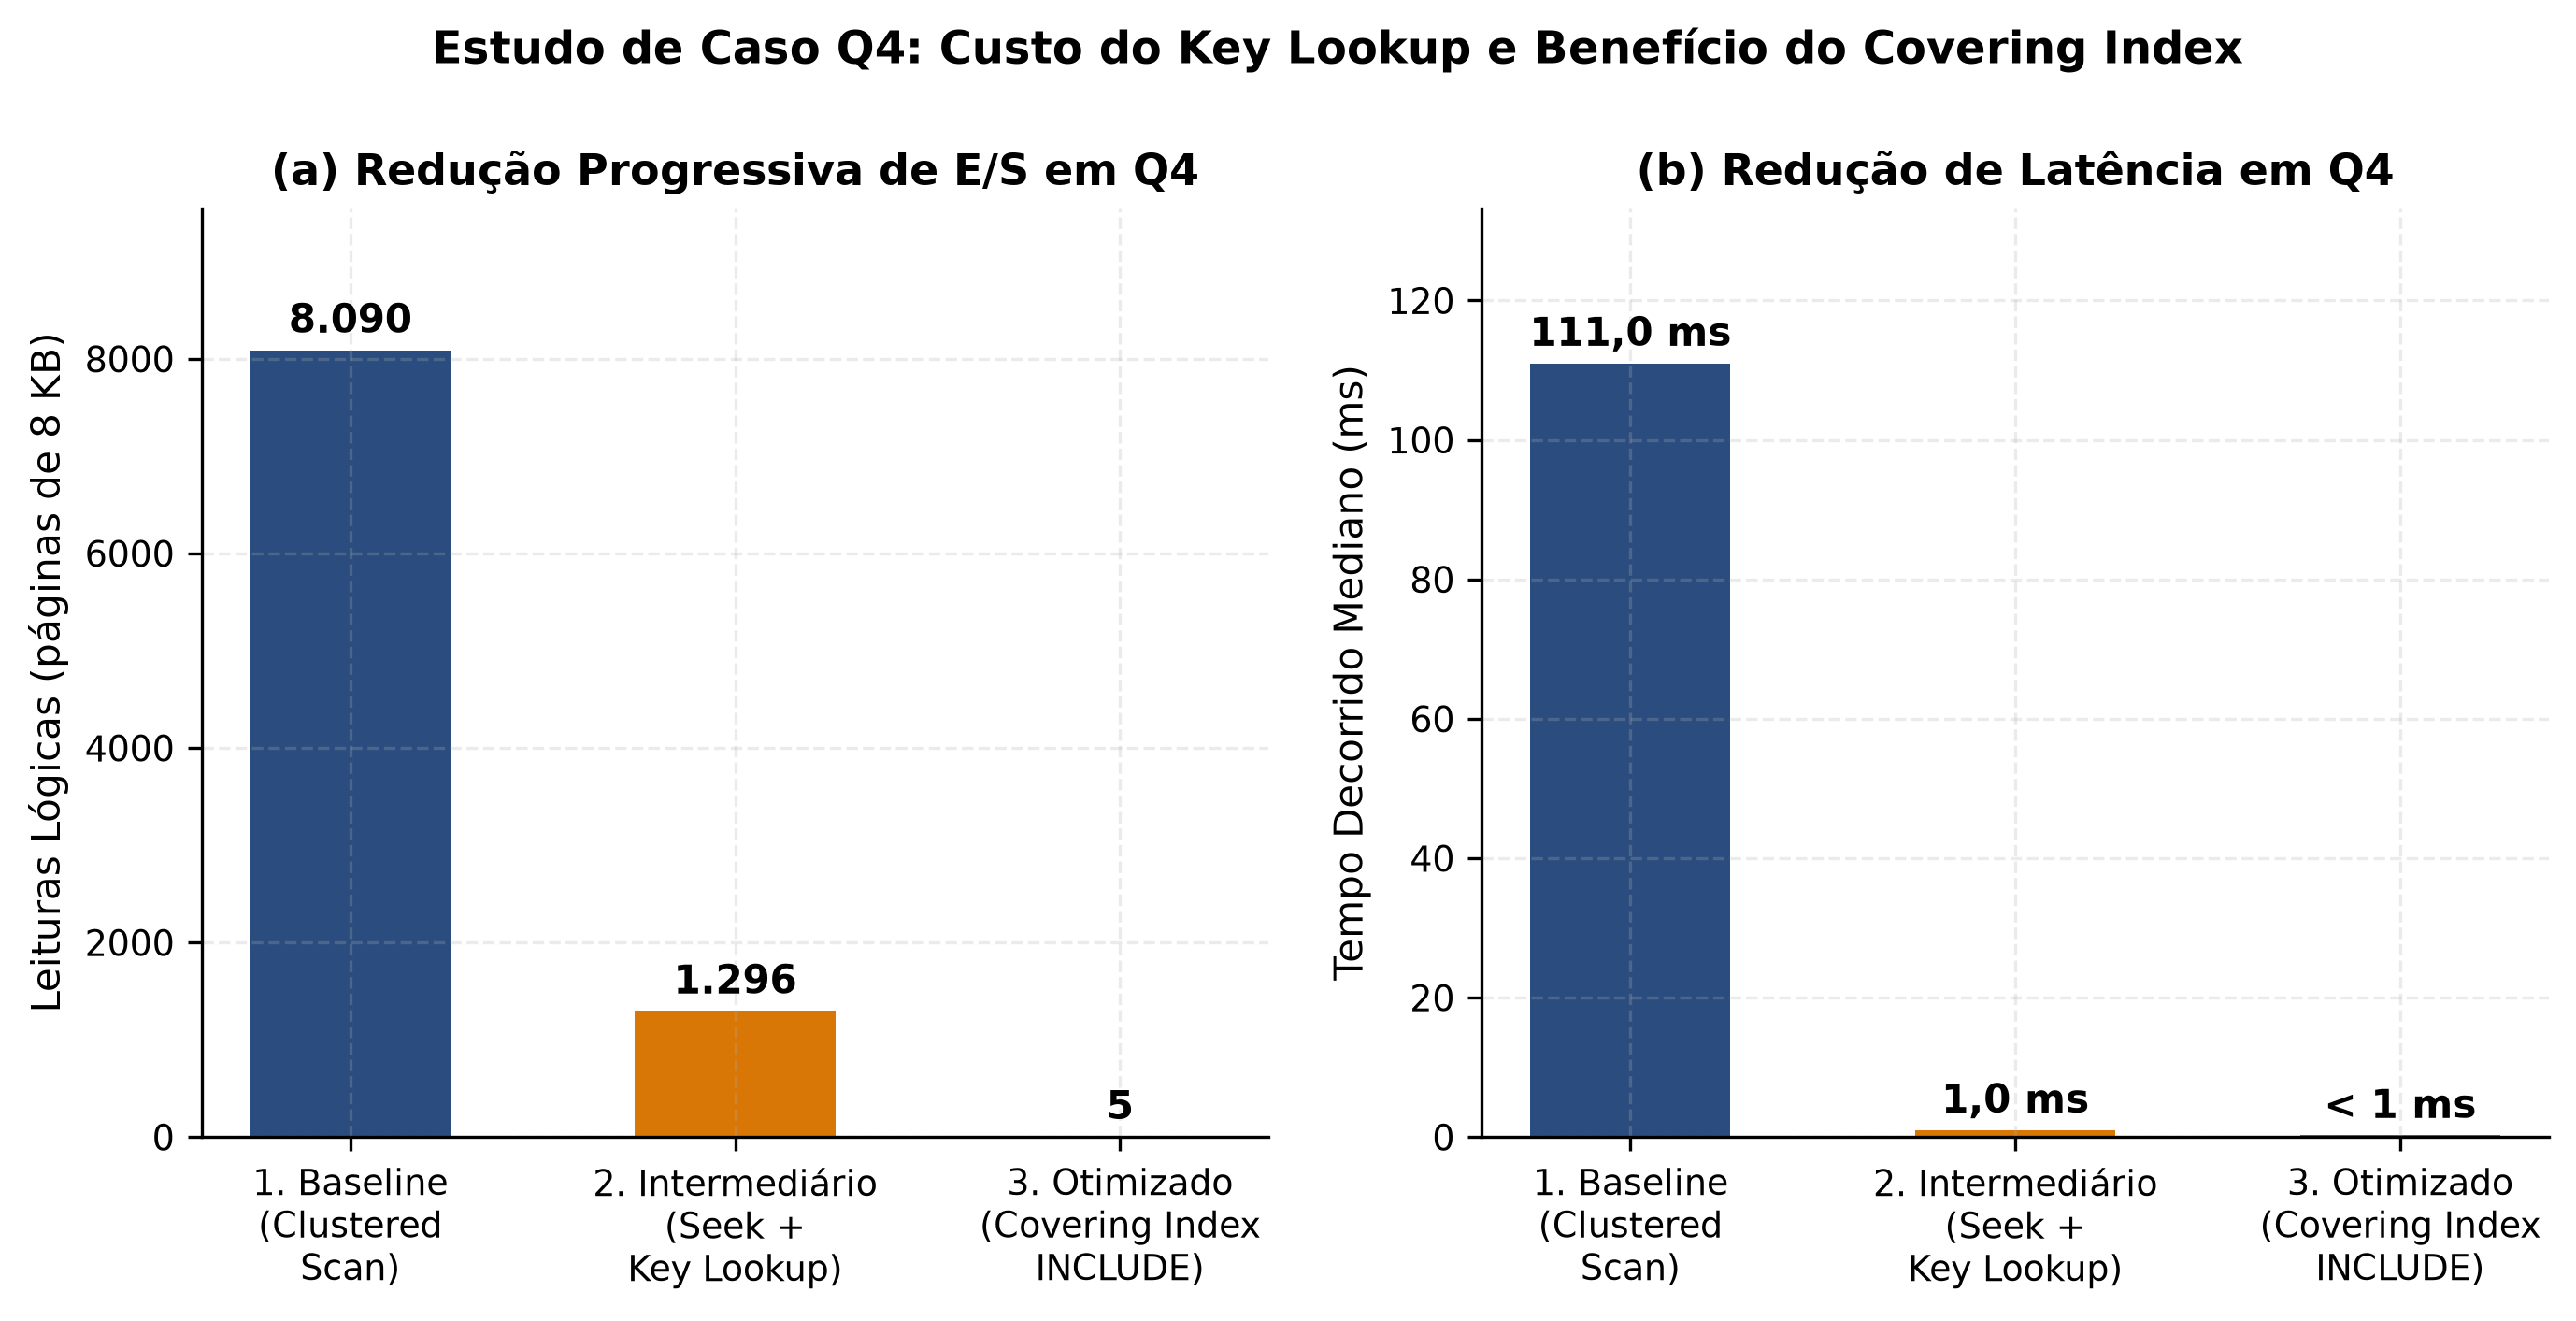
\includegraphics[width=0.78\textwidth]{figures/fig3_q4_tres_estagios.png}
\caption{Evolução em três estágios de $Q_4$: eliminação de 422 operações de \textit{Key Lookup} (1.296 para 5 leituras lógicas) via índice de cobertura com \texttt{INCLUDE}.}
\label{fig:q4-estagios}
\end{figure}

A inspeção direta das árvores de operadores extraídas dos arquivos \texttt{.sqlplan} (Figura~\ref{fig:planos-execucao}) sintetiza os quatro fenômenos arquiteturais centrais observados neste estudo: substituição de \textit{Clustered Scan} por \textit{Seek + Key Lookup} em $Q_1$ (a), remoção do \textit{Key Lookup} em $Q_4$ (b), troca de modo de execução vetorial em $Q_7$ (c) e multiplicação de escrita em $W_1$ (d).

\begin{figure}[htbp]
\centering
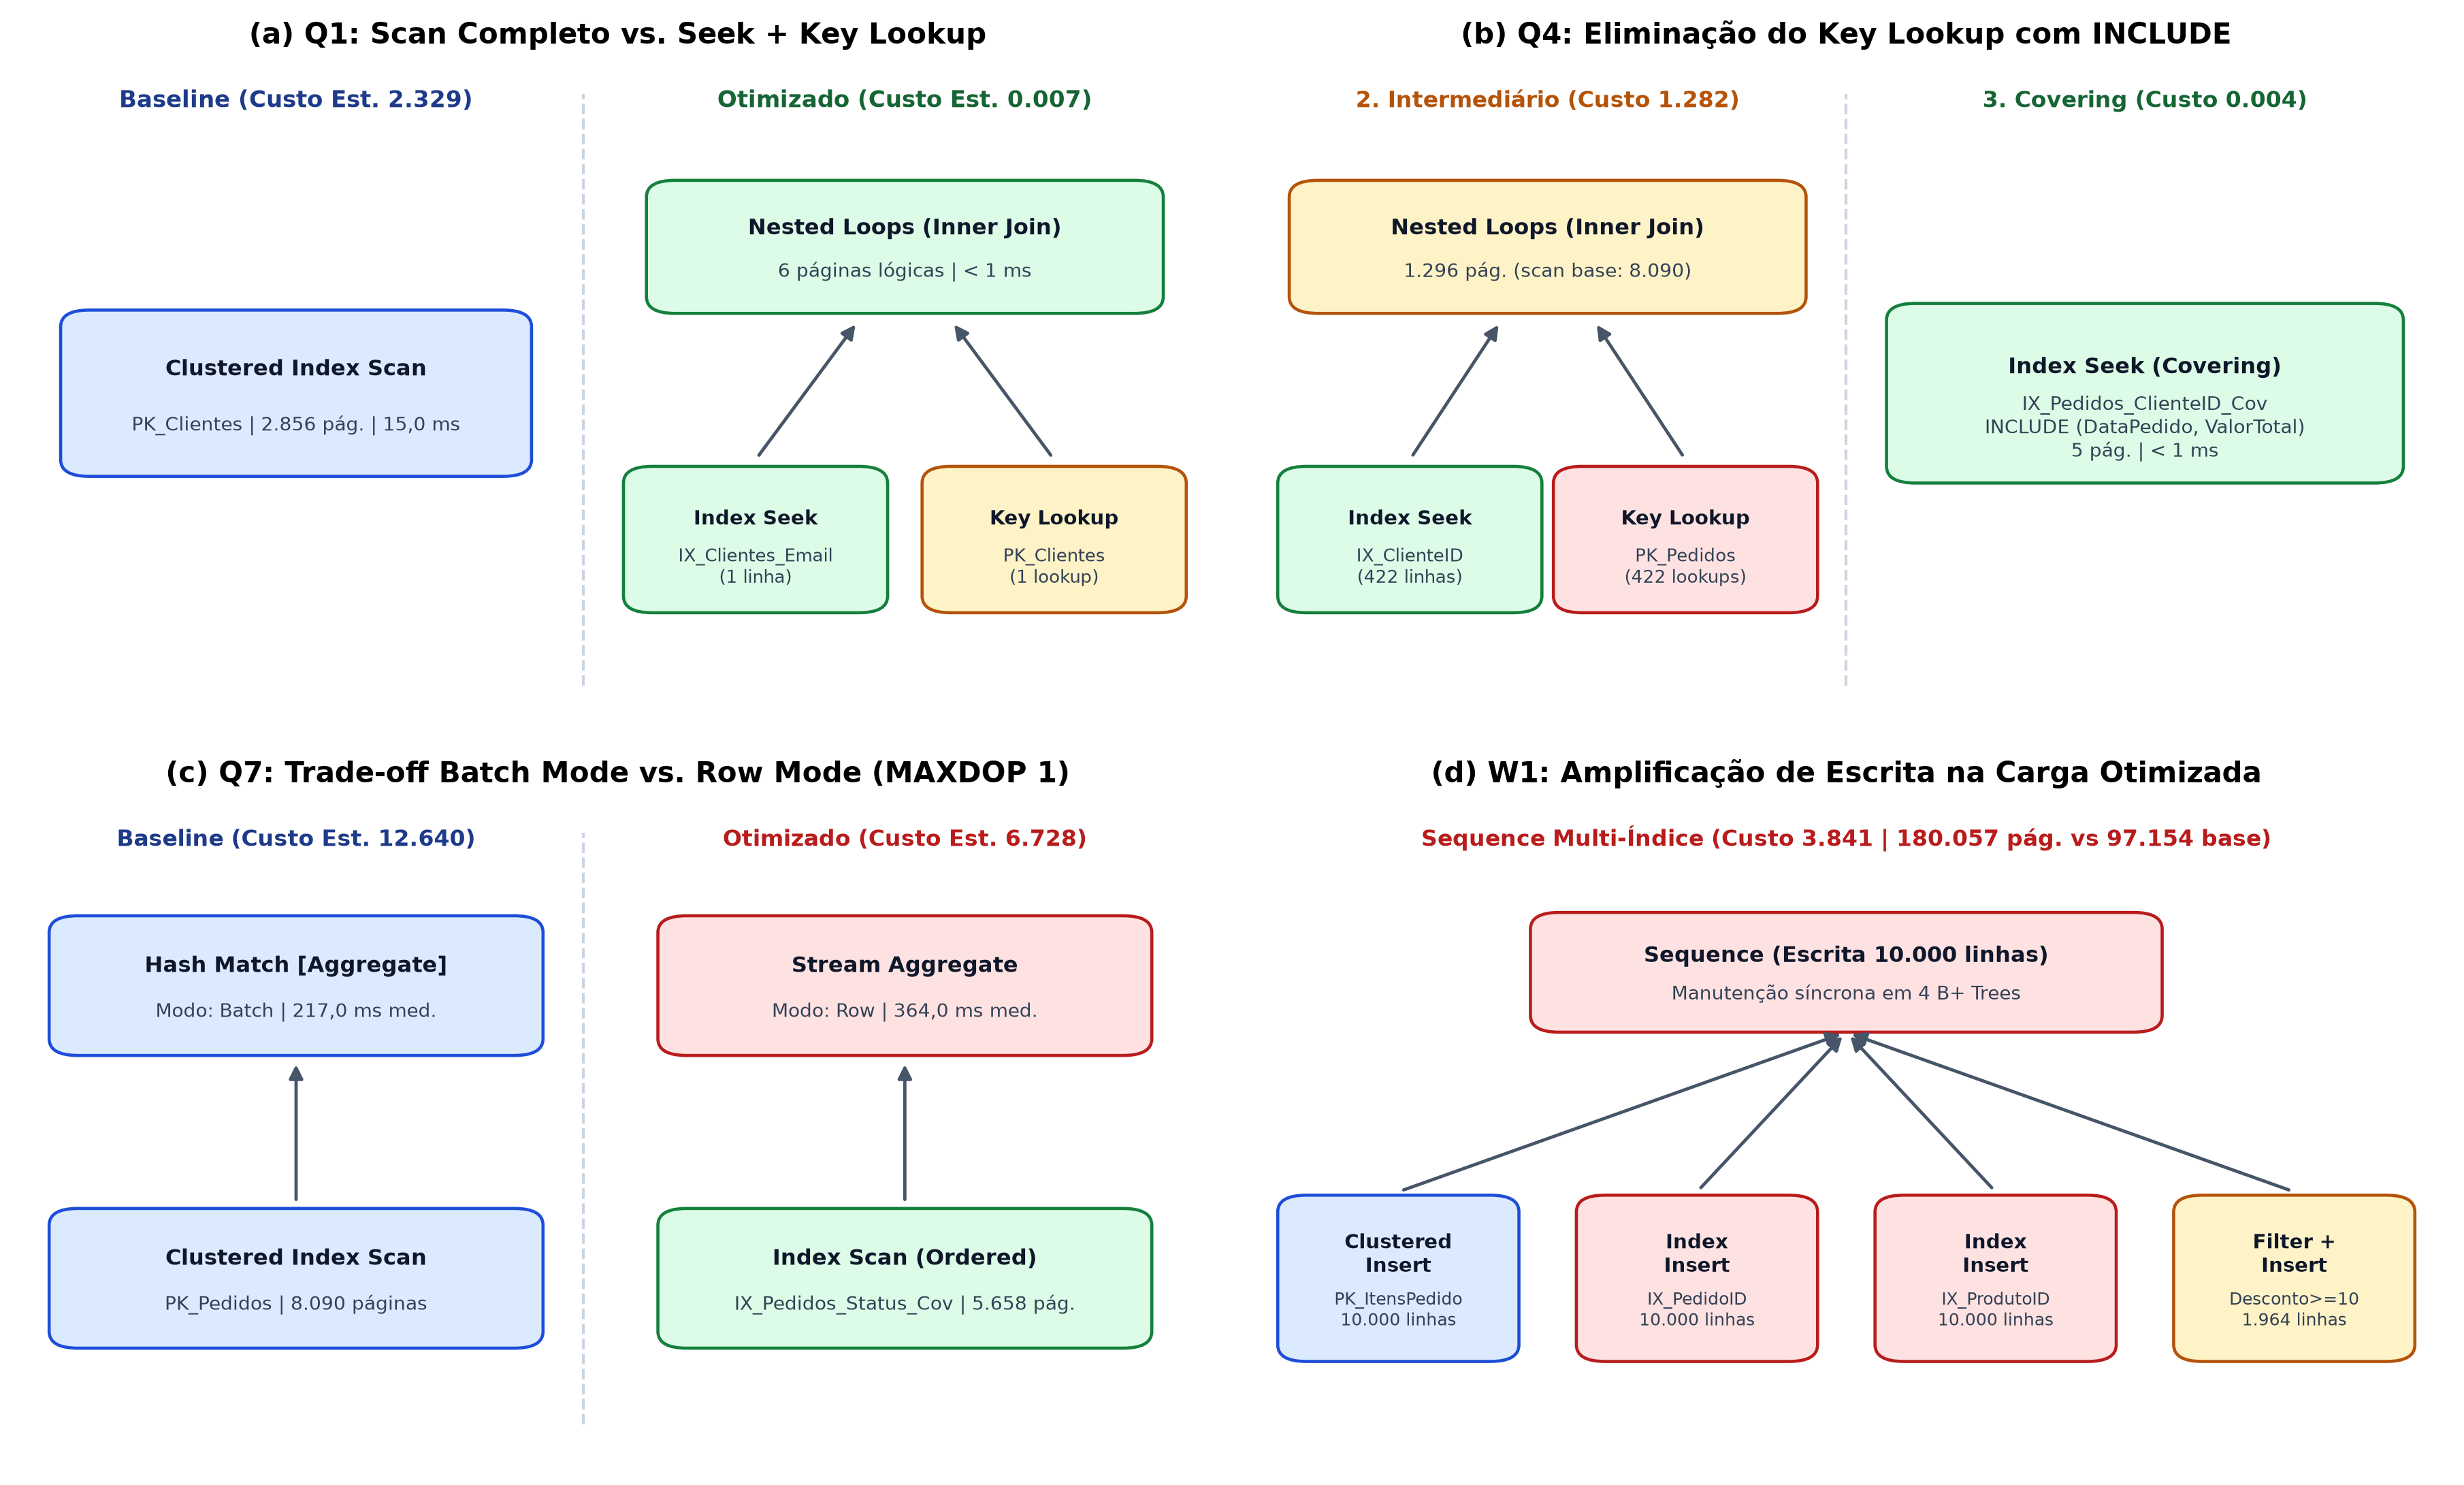
\includegraphics[width=0.82\textwidth]{figures/fig5_planos_execucao.png}
\caption{Diagramas comparativos dos planos físicos reais extraídos dos XML (\texttt{ShowPlanXML}) para $Q_1$, $Q_4$, $Q_7$ e $W_1$, com custos estimados e leituras observadas.}
\label{fig:planos-execucao}
\end{figure}

\subsection{Trade-offs: \textit{Batch Mode} vs. \textit{Row Mode} ($Q_7$), Escrita ($W_1$) e Cache}

Dois resultados negativos ou mistos merecem análise aprofundada, pois ilustram limites reais que análises puramente simplistas de índices costumam ocultar:

\begin{enumerate}
\item \textbf{Inversão de Latência em $Q_7$ (\textit{Batch Mode} vs. \textit{Row Mode}):} Embora o índice de cobertura \texttt{IX\_Pedidos\_Status\_Cov} tenha reduzido as leituras lógicas de 8.090 para 5.658 (-30,06\%) e eliminado o consumo de memória de tabela \textit{hash}, o tempo mediano aumentou de 217,0~ms para 364,0~ms em \textit{Warm Cache} (\textit{speedup} $0{,}60\times$, $p < 10^{-4}$) e de 402,0~ms para 685,0~ms em \textit{Cold Cache} ($0{,}59\times$). A inspeção dos atributos \texttt{ActualExecutionMode} no \texttt{ShowPlanXML} (Figura~\ref{fig:planos-execucao}c) esclarece a causa: no Baseline, o otimizador estimou custo de subárvore de 12,640 usando \textit{Clustered Index Scan} + \textit{Hash Match}, acionando automaticamente o motor vetorizado \textbf{\textit{Batch Mode on Rowstore}} sobre as 1,5 milhão de linhas; na base otimizada, atraído pelo menor custo estimado (6,728) e pela ordenação prévia de \texttt{Status} no índice estreito, escolheu \textit{Index Scan} + \textit{Stream Aggregate}, que operou em \textbf{\textit{Row Mode}} tupla-a-tupla, acumulando maior sobrecarga de CPU por linha sob \texttt{MAXDOP 1}.

\item \textbf{Amplificação de Escrita em $W_1$:} Na inserção em lote de 10.000 registros em \texttt{ItensPedido}, a base Baseline manteve apenas a árvore clusterizada (\texttt{PK\_ItensPedido}), consumindo 97.154 leituras medianas em \textit{Warm Cache} (77.448,5 em \textit{Cold Cache}). Na base otimizada, o plano exibiu um operador \texttt{Sequence} executando quatro gravações em árvore B+: a inserção clusterizada e três \texttt{Index Insert} secundários (\texttt{IX\_ItensPedido\_PedidoID}, \texttt{IX\_ItensPedido\_ProdutoID} e o índice filtrado \texttt{IX\_ItensPedido\_Desconto\_Alto}, que atuou seletivamente sobre 1.964 das 10.000 tuplas inseridas). Como resultado, as leituras lógicas saltaram para 180.057 em \textit{Warm Cache} (+85,33\%, latência com variância elevada de 404,0 $\pm$ 853,2~ms, $p = 0{,}129$) e para 282.476 em \textit{Cold Cache} (+264,73\%, com tempo subindo de 502,0 para 1.098,5~ms, $0{,}46\times$, $p = 0{,}00195$).
\end{enumerate}

Por fim, a Figura~\ref{fig:warm-cold} contrasta os regimes \textit{Warm} ($N=30$) e \textit{Cold} ($N=10$) para seis consultas representativas. O esvaziamento explícito do \textit{buffer pool} e do cache de planos impôs penalidades severas tanto de compilação quanto de \textit{read-ahead} físico: $Q_1$ otimizada passou de $<1$~ms para 3,5~ms (ainda $12{,}6\times$ mais rápida que o Baseline frio de 44,0~ms); $Q_5$ otimizada subiu de 12,0~ms para 237,5~ms devido às leituras aleatórias de páginas frias em \texttt{ItensPedido} (11.927,5 leituras lógicas frias), mantendo porém sólida vantagem sobre os 1.027,5~ms do Baseline frio ($4{,}33\times$). Em todas as 220 execuções \textit{Cold Cache} registraram-se \texttt{physical\_reads >= 1}, confirmando que as diferenças refletem leitura real fora do \textit{buffer pool}.

\begin{figure}[htbp]
\centering
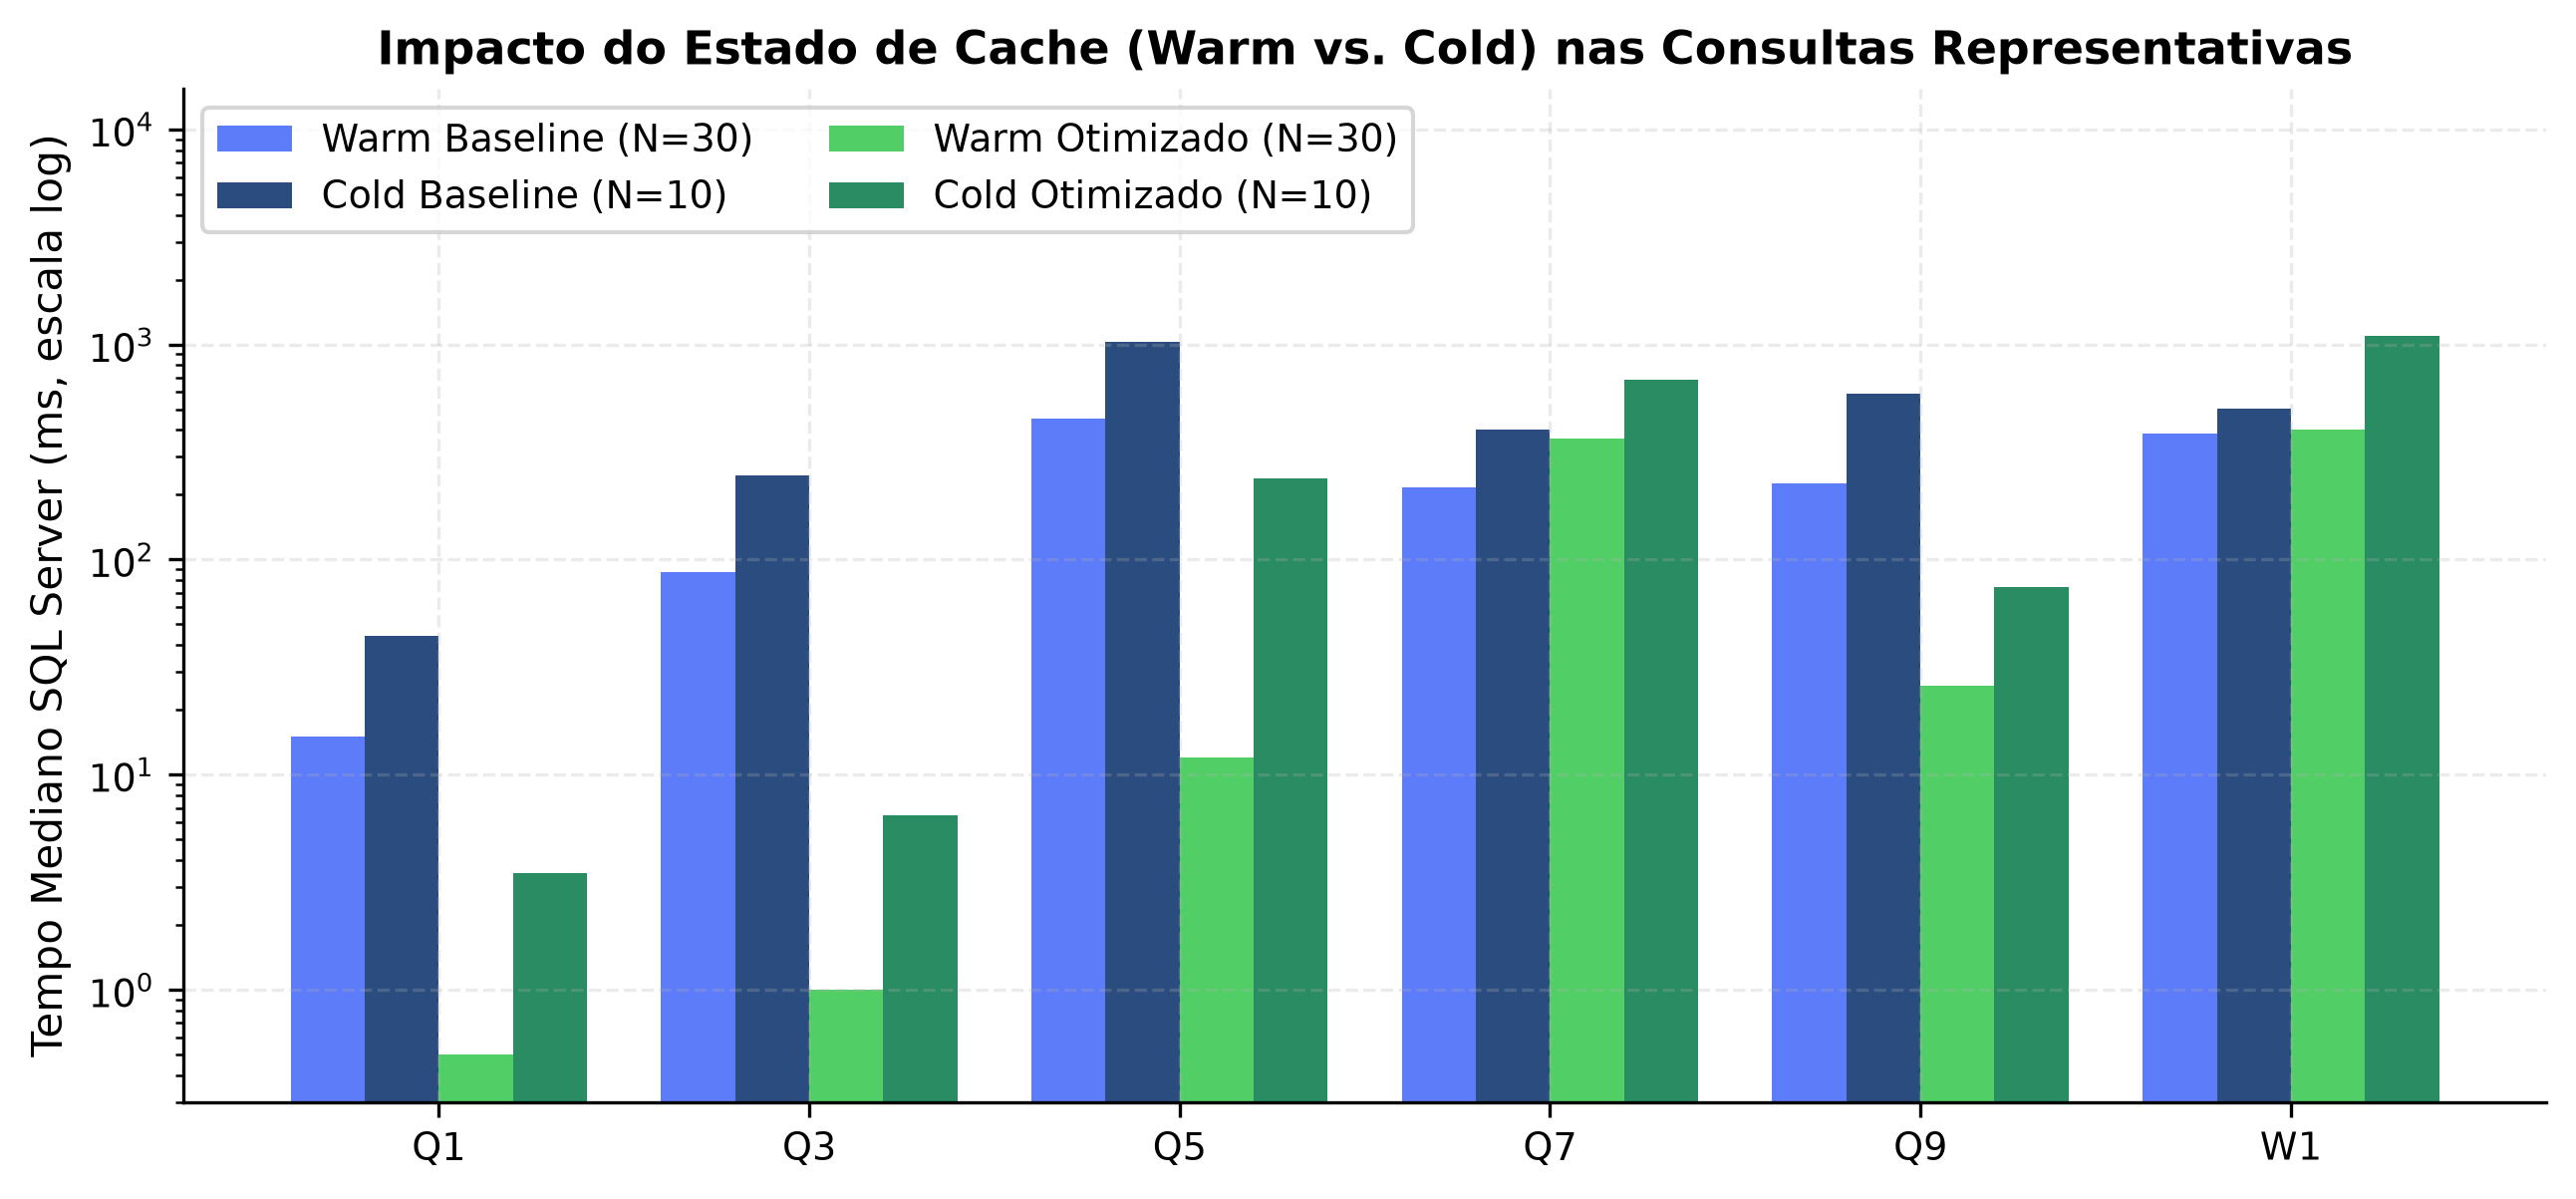
\includegraphics[width=0.76\textwidth]{figures/fig4_warm_vs_cold_cache.png}
\caption{Impacto do estado de cache (\textit{Warm Cache} $N=30$ vs. \textit{Cold Cache} $N=10$) nas consultas representativas em escala logarítmica.}
\label{fig:warm-cold}
\end{figure}

\section{Conclusão}

Este estudo demonstrou experimentalmente, em um cenário de 6,25 milhões de registros no Microsoft SQL Server 2022, que a combinação disciplinada de índices B+ e reescrita SQL produz ganhos substanciais e estatisticamente significativos na vasta maioria das cargas de leitura: reduções de E/S lógica de até 99,96\% ($Q_6$), eliminação de \textit{Key Lookups} com redução de 1.296 para 5 páginas ($Q_4$), substituição de \textit{Hash Joins} custosos por \textit{Merge Join} e \textit{Nested Loops} ($Q_5$, $37{,}5\times$) e recuperação de sargabilidade em predicados textuais ($Q_8$, $114{,}0\times$) e temporais ($Q_9$, $8{,}69\times$).

Contudo, os dados empíricos refutam a premissa simplista de que ``mais índices ou menor E/S garantem sempre menor tempo de resposta''. A penalidade de escrita de +85,33\% em leituras lógicas ($W_1$) comprova que cada índice secundário impõe custo síncrono em cargas OLTP intensivas, enquanto o comportamento de $Q_7$ demonstra que otimizadores baseados em custos podem trocar planos vetorizados em \textit{Batch Mode} por agregações escalares em \textit{Row Mode}, degradando a latência em 67,7\% apesar da economia de 30\% em páginas lidas.

Como limitações (\textit{threats to validity}), destaca-se que os testes foram conduzidos com \texttt{MAXDOP 1} em container único no mesmo disco SSD do \textit{host} (sujeito ao cache de páginas do sistema operacional durante \textit{Cold Cache}). Como trabalhos futuros, planeja-se avaliar planos paralelos multi-thread, índices colunares (\textit{Columnstore}) para consultas analíticas do tipo $Q_7$ e cargas mistas concorrentes de leitura e escrita simultânea.

\bibliographystyle{sbc}
\bibliography{sbc-template}

\end{document}
